\documentclass[a4paper,twoside,openleft,12pt]{filipecorreiathesis} % define the title 
\usepackage[a4paper,margin=2.5cm, top=3cm, bottom=3cm]{geometry} % use bindingoffset=2cm for binding
\usepackage{appendix}
\usepackage{makeidx}
\usepackage{fancyhdr}
\usepackage{amsfonts, amssymb, amsthm, mathrsfs}
\usepackage{multicol}
\usepackage{multirow}
\usepackage{setspace} 
\usepackage{xspace}
\usepackage{algorithm, algorithmicx, algpseudocode}
\usepackage{rotating}
\usepackage{courier}
\usepackage{textcomp}
\usepackage{booktabs}
\usepackage{bookmark}
\usepackage[ISBN=555-555-555-555-0,SC0]{ean13isbn}
\usepackage{wrapfig}
\usepackage{soul} % provides yellow-marker highlighting among other features
\usepackage{verbatim} % provides the 'comment' environment among other features
\usepackage{xifthen} % provides \ifthenelse 

\usepackage{enumitem}
\usepackage{pbox}
\usepackage[section]{placeins} % stops floats (figures, tables...) to appear outside the section where they are placed.
\usepackage{cleveref}[2012/02/15]

\usepackage{longtable}
\usepackage{subcaption}

\usepackage{calligra}
\newcommand{\setfont}[2]{{\fontfamily{#1}\selectfont #2}}

\usepackage[]{todonotes}
\presetkeys%
    {todonotes}%
    {inline,backgroundcolor=yellow}{}

\makeindex

% dividing diamonds
\newcommand{\dividingdiamonds}{\vspace{0.2cm}\centerline{$\diamond \diamond \diamond$}\vspace{0.2cm}}%


%\onehalfspacing
\setstretch{1.3} % for custom spacing

% indentation of multiline figure/table captions.
%\usepackage[format=plain,justification=RaggedRight]{caption}

% Vertically centered table columns
\newcolumntype{M}{>{\centering\arraybackslash}m{\dimexpr.25\linewidth-2\tabcolsep}}

%% Fixes problem with bibliograpy key protruding into description
\usepackage{eqparbox}
\usepackage[numbers]{natbib}
\renewcommand*{\bibnumfmt}[1]{\eqparbox[t]{bblnm}{[\textcolor{feup}{#1}]}}

\def\isnum#1{%
  \if!\ifnum9<1#1!\else_\fi
    \oldstylenums{#1}\else#1\fi}

%% Fancy Headers -- Somehow, I can't seem to be able to move this to the .cls file
\pagestyle{fancy}
\fancyhf{}
\fancyhead[LE]{\small \leavevmode\llap{\textcolor{feup}{\isnum{\thepage}}\hspace{0.5cm}}\smallcaps{\leftmark}}
\fancyhead[RO]{\small \leavevmode\smallcaps{\rightmark}\rlap{\hspace{0.5cm}\textcolor{feup}{\isnum{\thepage}}}}
\fancypagestyle{plain} {
 \fancyhf{} % get rid of headers on plain pages
 \renewcommand{\headrulewidth}{0pt} % and the line
 \renewcommand{\footrulewidth}{0pt} % and the line
}
\renewcommand{\headrulewidth}{0pt}
\renewcommand{\footrulewidth}{0pt}
\setlength\headsep{1.1cm}
\setlength\headheight{13.6pt}

\renewcommand{\chaptermark}[1]{\markboth{#1}{}}
\renewcommand{\sectionmark}[1]{\markright{#1}{}}

%% Define a new 'leo' style for the package that will use a smaller font.
\usepackage{url}
\makeatletter
\def\url@leostyle{%
  \@ifundefined{selectfont}{\def\UrlFont{\sf}}{\def\UrlFont{\footnotesize\ttfamily}}}
\makeatother
\urlstyle{leo}

%\usepackage{inconsolata} % monospace font, used for \texttt{}


\begin{document}
	\title{TESThesis }
	\author{\href{mailto:your-email-address@fe.up.pt}{Pedro Miguel Lourenço Costa}}

	\frontmatter
	    \pagestyle{empty}
	    \maketitle
		\noindent\textbf{Contact Information:} \\

\noindent Pedro Miguel Lourenço Costa \\
Faculdade de Engenharia da Universidade do Porto \\
Departamento de Engenharia Informática \\

\noindent Rua Dr. Roberto Frias, s/n \\
4200-465 Porto \\
Portugal \\

\noindent Tel.: +351 968 203 386 \\
Email: pedro.miguel.costa@fe.up.pt \\
URL: https://www.linkedin.com/in/pedro-costa-3279996b \\

\vfill


		\cleardoublepage
		\begin{flushright} 
  %\null\vspace{\stretch{1}}
  \null
  \vfill
  \emph{\Large{\dots to the world in general}} \\
  \vspace{3cm}
\end{flushright}
		\clearpage
		{\centering \emph{This page was intentionally left blank.} \\ }
		\dominitoc
		\cleardoublepage
		\pagenumbering{roman}
		\pagestyle{fancy}
		\chapter{Abstract}


Nowadays, nearly every medium-size or large company in the electronics, pharmaceutics, food, or other industries needs to support its operations by managing the exchanged information and resources. The upstream and downstream flow of these, together with the system of organizations, people and activities that make it possible, is commonly referred to as a supply chain. In a practical sense, a supply chain’s flow of products and services goes from supplier to consumer. For example, the supermarket fish a person eats: it is caught in boats, then prepared, and distributed to a store where the final consumer is able to buy it. But supply chains are becoming very complicated and complex systems, spanning multiple businesses and relationships, interlaced in many different ways, which is a reason why supply chain management (SCM), the discipline which deals with the coordination of a supply chain, is becoming increasingly more important.  The information has to flow through the chain, sometimes even reverting the direction, but the paths it takes are not always very obvious or even traceable in the global context, dealing with many issues along the way.

Managing inventory and suppliers while maintaining safety, quality and keeping to the schedule is a difficult task. Delays are common, and a company’s finances, growth and reputation are affected. This is further aggravated by the fact that information is not always accurate or available when needed. And the fact that companies value their privacy makes it so that sharing information with others is not always simple or desirable. 

Most important of all, frequently, there are big holes of information in a supply chain, analog gaps where the information has not been made digital in the system. The use of traditional tools is still too prevalent. Emails are sent, documents are printed and mailed, instead of making the information digital, putting  it directly on the network and relaying it to the next link in the chain. This fact, together with the sometimes apparent lack of interoperability between the SCM software of different companies and their need to protect their private information is what makes a global overview of the whole chain complicated with the current technologies. Provenance and traceability of a supply chain are a big objective for companies, along with improving security, efficiency and effectiveness of the supply chains.

Most of these issues are, in great part, caused by the standalone use of outdated or inadequate software architectures, which, traditionally, are often centralized and have single points of failure. And even when they are not, oftentimes they are insecure, prone to synchronization problems, leading to big delays in both relaying the information and resources and making payments possible. 

One way to approach these specific problems of supply chains that are brought by the traditional IT solutions is to update them with new infrastructures, namely by using blockchain technology. Blockchain is a decentralized technology that has no single point of failure and allows for the immutable storage of verifiable data all over the computers that store it. Each time there is a new piece of information, its validity is verified by the network and it is inserted into a block of the chain, which leads it to being continually extended. This means that we can check all the information that there ever was, since the beginning, and validate it easily, or make any necessary calculations. As such, blockchains are the perfect means to achieve traceability of a supply chain. At the same time they are a secure and incorruptible way to store information, with a fast synchronization time, being perpetually available to anyone, anywhere within the network. It would also be the way to close the analog gaps, turning the chain fully digital, leading to the possibility of a global overview.

This project focuses on researching the effects of applying blockchain technology to a supply chain and its management. By doing this, it should be possible to ascertain how much this technology can really impact SCM over the traditional IT solutions, or in combination with them. A practical instance involving the application of this technology to a system will also be developed, to further demonstrate its possible benefits.

The improvements that it could bring are, however, not limited to the problems described. Blockchain is a whole new game, and it brings a whole new myriad of possibilities into the table. We are only seeing the tip of the iceberg and this is an area that is of the interest of any company which aims to improve the efficiency and effectiveness of its entire supply chain system.

\textbf{Keywords:} Supply Chain, Supply Chain Management, Industry, Blockchain, Network, Decentralization, Security, Traceability, Provenance, Information Integration, Ledger, Interoperability


\chapter{Resumo}

Tradução PT do abstract





		\addtocontents{toc}{\protect{\pdfbookmark[0]{\contentsname}{toc}}}
		\tableofcontents
		\cleardoublepage
		\phantomsection
		\addcontentsline{toc}{chapter}{\listfigurename}
		\listoffigures
		\cleardoublepage
		\phantomsection
		\addcontentsline{toc}{chapter}{\listtablename}
		\listoftables
		\cleardoublepage
		\chapter{Preface}

\epigraph{\emph{
A quote
}}{\sc The Quote's Author}
\vspace{1pc}


Lorem ipsum



	\mainmatter

	% final lineup
	%\chapter{Introduction1}
%\minitoc \mtcskip \noindent
%\chapter{Introduction2}
%\minitoc \mtcskip \noindent
\chapter{Introduction}
\label{chap:introduction}
\minitoc \mtcskip \noindent

Our society is turning more consumerist, with most people in developed countries having high consumer power and standards of life. Consumers goods, from the essentials up until the entertainment goods, are manufactured and ordered continuously in high quantities.

Modern supply chains feel the pressure of this growth, leading to the demand for an efficient management. Most companies are making efforts towards this end, and, even though part of the answer to an efficient management lies in having efficient processes, a good management is also based in using the right technologies. Thus, the development of technologies that can satisfy the demands of supply chain management, for any industry, is in high demand.

%The development of such technologies should be faced towards the problems that supply chains 

%ace concerns are raised as to whether the demand can be met in a transparent and trustful way. It is difficult to know where the products we consume come from, and the processes they go through. This leads to the need of transparency in the supply chains as well as the need of an increase in their efficiency, if they are to conform to the market's needs.

\section{Supply Chains}
\label{supply_chains}
\textbf{Supply Chains} can be found, in some form, in nearly every business, spanning many different areas of operation. Traditionally, a supply chain encompasses all the processes and activities that lead from the initial raw materials to the final finished product, as well as all the functions and services within and outside a company. A supply chain can also be defined as the network of entities through which material flows. These entities can be identified as suppliers, carriers, manufacturing sites, distribution centers, retailers, and customers~\cite{Lummus2014}. Naturally, with the upstream and downstream flow of these materials and resources, comes a lot of information on them and on the processes, people and organizations they are associated with. Realistically, the  flow is not always arborescent, as there are many considerations to be taken and decisions to be made. Supply chains have multiple end products with shared components, facilities and capacities~\cite{Ganeshan1995}. As a consequence, the paths taken by the resources and information are not straightforward, but interlace, diverge and converge at different points, go back and forth, as exemplified in Figure~\ref{fig:supplychain_complexity}.
  
\begin{figure}[ht]
\centering
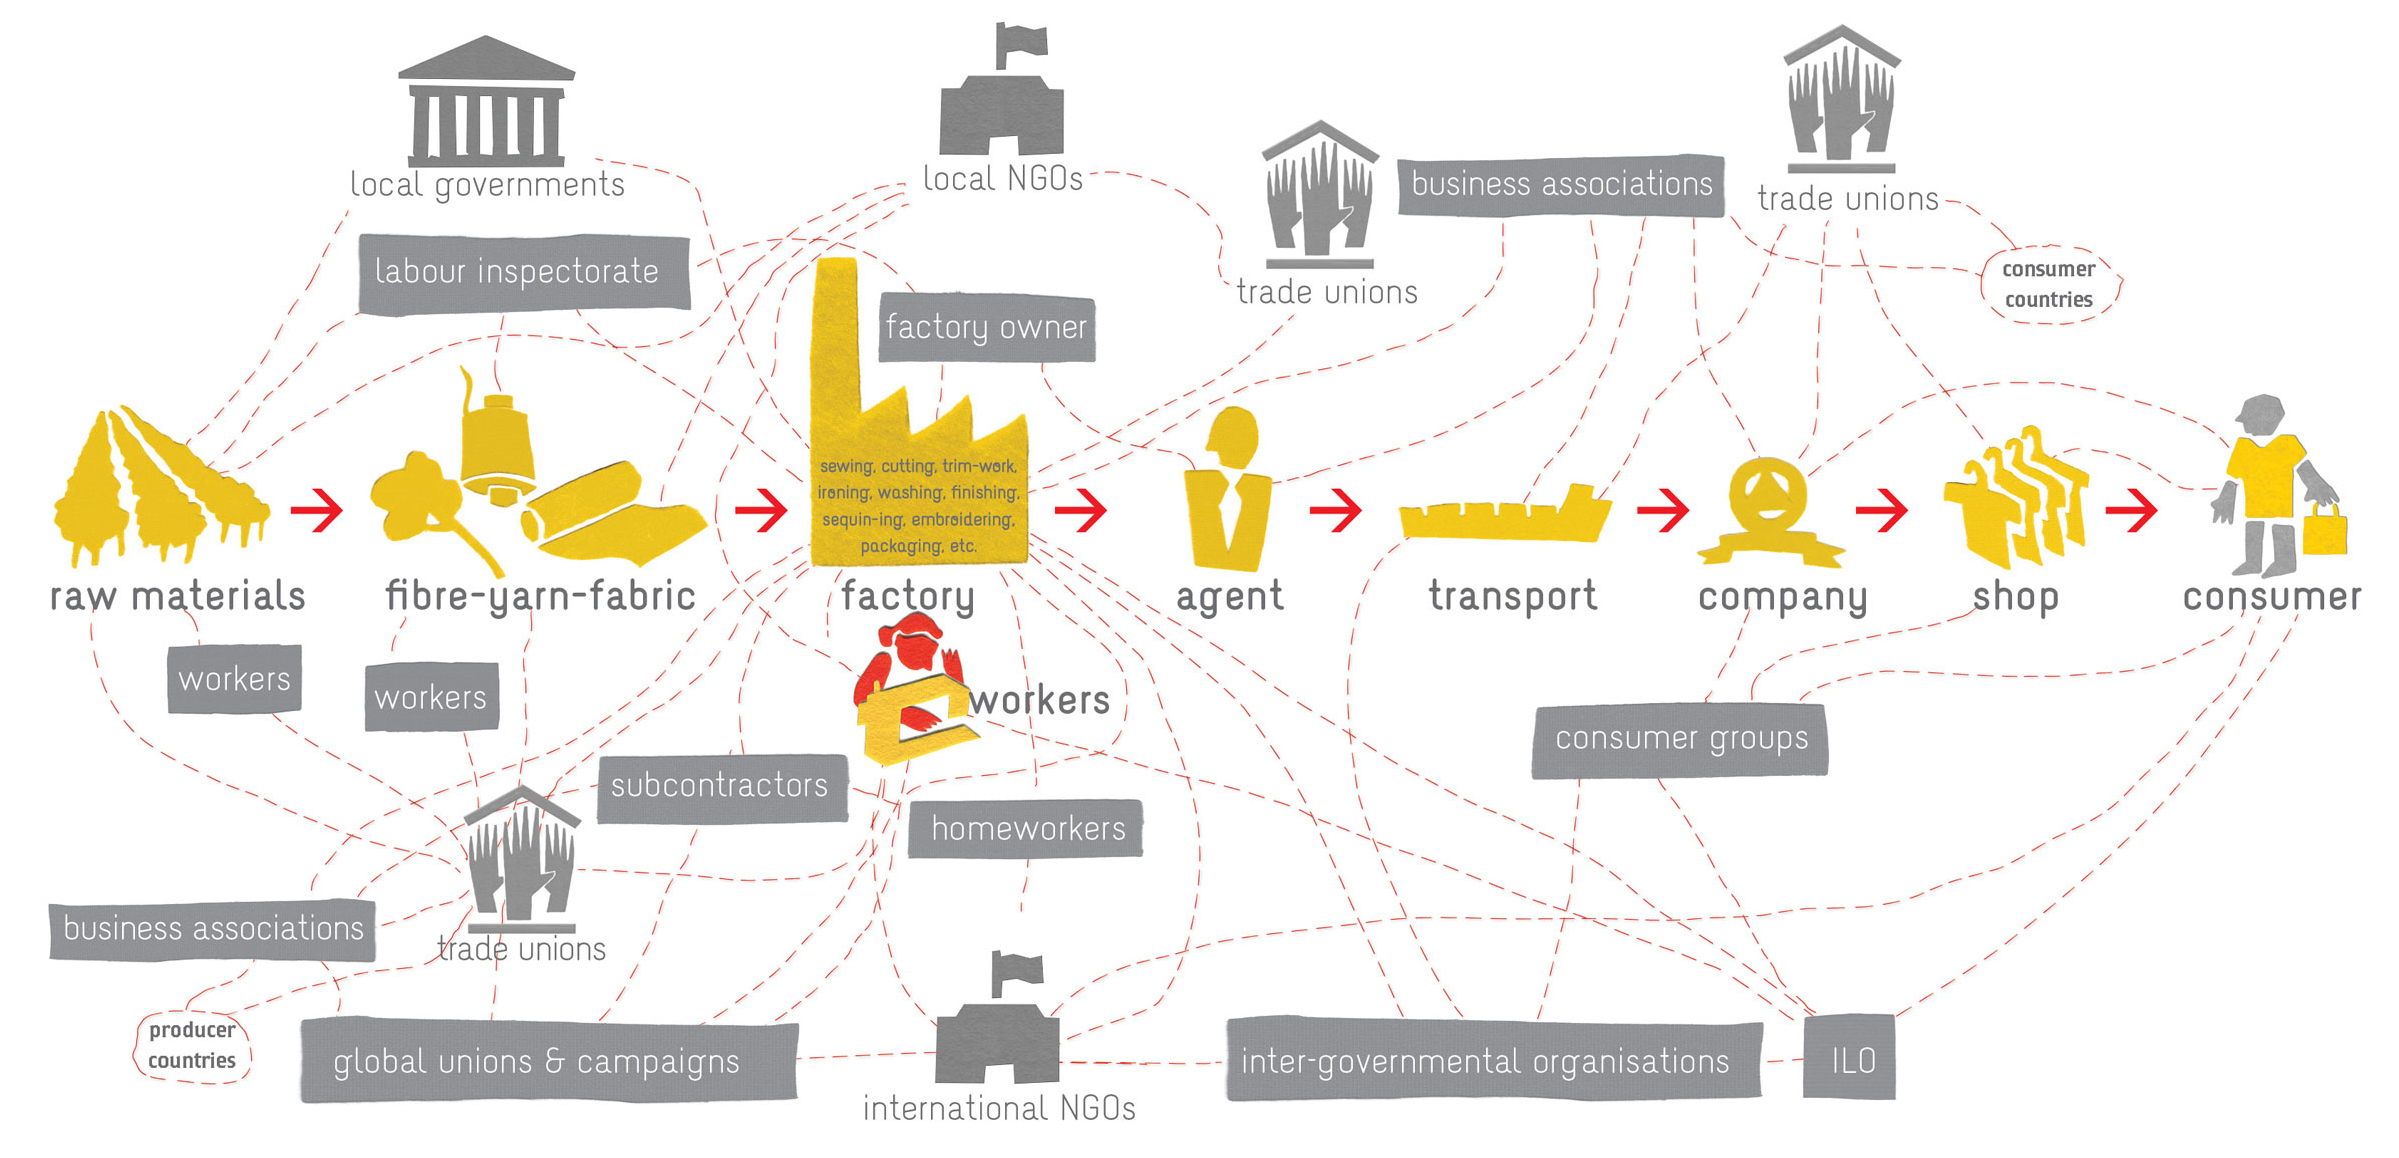
\includegraphics[scale=0.18]{media/supplychain_complexity.jpg}
\caption[Representation of a garment supply chain and all the relationships it involves]{Representation of a garment supply chain and all the relationships it involves. Taken from the International Training Centre of the International Labour Organization briefing on global supply chains~\cite{ITCILO2018}.}
\label{fig:supplychain_complexity}
\end{figure}
  
  The activities and processes a supply chain encompasses include: sourcing raw materials and parts, manufacturing and assembly, warehousing and inventory tracking, order entry and order management, distribution across all channels, delivery to the customer, and managing the information systems necessary to monitor all of these activities. As Lummus~\cite{Lummus2014} describes, these activities can be roughly mapped to the 4 essential processes: plan, source, make, deliver.
    
  Coordinating all of these is no easy task, and so the discipline of SCM comes into life. According to Ballou~\cite{Ballou2007}, the Council of SCM Professionals (CSCMP) defines SCM as \textit{“the planning and management of all activities involved in sourcing and procurement, conversion, and all Logistics Management activities. Importantly, it also includes coordination and collaboration with channel partners, which can be suppliers, intermediaries, third-party service providers, and customers. In essence, SCM integrates supply and demand management within and across companies”}.

From this definition follows that SCM deals a lot with both coordination and collaboration between entities, and so, the management of the flow of information and resources between them is very important. The objective is always, of course, to minimize the total cost of these flows between and among stages~\cite{Habib2011}.
In the end, the creation of value (products and services) in a supply chain stems from the relationships that different entities build between themselves, and not from the work of a single entity. As such, supply chains, not firms, compete and those which have the best integration and management processes win.

And this is where SCM shines and shows just how useful it can be. Managing all the processes in a supply chain, while maintaining safety, quality and keeping to schedule is difficult. An event on one side of the world, large or small, be it from human or natural causes, can easily disrupt the links in the supply chain. For instance, it might disrupt the supply of a critical component or service. Delays are, therefore, common, and the consequences of such disruptions might have a severe impact in the finances, growth and reputation of the companies involved~\cite{Punter2013}.

SCM diminishes the impact of such disruptions, and actively works to avoid or diminish them, while optimizing the way the supply chain works. This is why SCM is such an important discipline, that we have to better understand and improve, with all the means that we can, and this includes, of course, research into technologies like the blockchain.

\section{Challenges}
\label{sec:supply-chain-challenges}

 Having already introduced the concepts of Supply Chain and SCM, it is now possible to briefly introduce some of the problems that affect them.

The first, and most generalist problem of a supply chain, is the ease with which \textbf{an unexpected event might cause delays}. These events, already mentioned in Section~\ref{supply_chains} are not always predictable and must be contained as fast as possible. One event in particular which, often, causes delays are \textbf{synchronization problems in the processes and information systems of a company}~\cite{Prokle2017}. 

    Another problem is that, often, there are difficulties in sharing information between companies. This is caused both by the fact that \textbf{companies value their privacy and the security of their information}, which means they might not want to share too much information, or that they might only share it through secure channels, and by the \textbf{lack of standards for sending information and communicating}~\cite{Korpela2017}. The issue with non-existing standards is that companies are left to discuss what details to share or not, wasting time and resources.

Most important of all, in the industry, \textbf{the use of traditional tools and manual work is still too prevalent}. Emails are sent, documents are printed and mailed, instead of transmitting the information in a more automatic, direct and secure way through the network. This point also brings the next problem of supply chains to light: the apparent lack of interoperability between certain softwares (which might be a byproduct of by the lack of standards).
 
 
Finally, provenance and traceability of the products on a supply chain are a big objective for companies. But \textbf{the current technologies used in supply chain only accomplish provenance and traceability in a limited scope}, as the information a certain entity possesses is usually also limited. And so, it is very hard for anyone to have a global overview of the supply chain.

Though it is not proven, it is be possible that some, if not most, of these issues in supply chain might be caused by the use of software architectures that do not allow for full data integration. An optimal supply chain should be as efficient and effective as possible, while being secure and satisfying all the traceability requirements. Perhaps, it is time to try out new solutions which replace or augment the existing ones, in such a way that supply chain management can better satisfy the needed requirements.

\section{From Blockchain Technologies to Supply Chains} \label{sec:context}

Blockchain technology allows for secure, public, distributed and decentralized systems. Though it was first proposed in its actual form by Satoshi Nakamoto~\cite{Nakamoto2008}, an anonymous group which published a white paper in 2008, this was not the first reference to such a technology. The first work on a cryptographically secured chain of blocks was described in 1991 by Stuart Haber and W. Scott Stornetta~\cite{Haber1991}, and further refined in 1992 by Bayer \& Haber, by incorporating Merkle trees~\cite{Bayer1993}. Since then, it has come a long way, sprouting multiple different uses and applications of the technology. Its characteristics make the development of distributed and permanently, globally available systems possible, which is a paradigm that is attracting the interest of various industries.

One area in particular where we believe blockchain could bring about great improvements is Supply Chain Management (SCM). SCM has seen an increase in complexity in the last few decades, due to the globalization of the market, with businesses interlacing in many different ways, their relations extending way beyond what they used to, as found by Filiz Isik~\cite{Isik2011}. This increase in complexity is somewhat hard to manage and some supply chains stretch and encompass so many businesses that, due to their software not being prepared for this, the information is not always transmitted from end to end, leaving holes of information in between the links that join each business, thus leading to a lot of chaos and uncertainty as to the state of the key items in the chain~\cite{Wilding1998}.

   This dissertation work will focus on supply chain management, and on how blockchains can possibly be applied to improve this area, leading to positive impacts in the logistics industry and eventually finding benefits for the consumer as well. 

%%%%%%%%%%%%%%%%%%%%%%%%%%%%%%%%%%%%%%%%%%%%%%%%%%%%%%%%%%%%%%%%%%%

\section{Motivation} 
\label{sec:motivation}

As described in section~\ref{sec:supply-chain-challenges}, a possible cause of these problems might be the use of software that can not keep up with the evolution of the requirements of modern supply chains. Today's supply chains have high standards for their requirements and even when the software works just fine, maybe it is not recent enough or it was not specified and built to satisfy these requirements. For instance, product falsification might be a huge issue nowadays in the supply chain, but maybe it was not rated as a high importance problem 15 years ago. Therefore, the software from 15 years ago complied with different requirements than the ones from today and was not built to handle that specific problem well. 

\textbf{Requirements evolve, and so should the technology, in order to support them.} There is an immediate need for solutions, which might either completely replace the previous ones, or augment them.

One way to approach these specific problems is to research what would a modern requirements specification for supply chain look like, and develop new technologies that are more accurately specified for the supply problem challenges in question. 

The characteristics of blockchain architectures seem to be a good solution for many of the identified problems in supply chain to be reduced or neutralized. These architectures are the perfect means to achieve traceability of a supply chain, and so, they are good to achieve provenance as well. At the same time they are a secure, incorruptible and immutable way to store information, with a fast synchronization time, being perpetually available to anyone who has permission, anywhere within the network. It would also be the way to close the analog gaps, turning the chain fully digital, leading to the possibility of a global overview.

\section{Objectives}
\label{sec:objectives}
The main objective of this dissertation is to find whether blockchain technology is a good fit to solve the most common problems of supply chain management, and also to find out the technological requirements of a modern supply chain. There are a multitude of small tasks that blockchain could automatize in supply chain, so this thesis will try to figure out which ones blockchain applies to better. 

The primary objective of this dissertation is determining if blockchain architectures can be successfully applied to supply chain management as an improvement towards the technologies that are already being used. For this purpose, it is necessary to conduct research on the supply chain issues and validate these, in order to propose a blockchain design that can target these issues successfully. 

\section{Dissertation Structure} \label{sec:struct}

Besides the introduction, this dissertation has 6 more chapters, divided into 2 parts.

\par \textbf{Part 1: Background and State of the Art} - Provides the needed concepts to understanding the work, as well as explanations about the existing tools and projects related to the blockchain and to its application to supply chain management domain.
 The state of the art is divided into 2 chapters:~\ref{chap:blockchain} and ~\ref{chap:blockchain-applicability}.
\begin{itemize}
  \item Chapter~\ref{chap:blockchain}, "Blockchain Technologies", some important concepts from the blockchain architecture are presented and discussed, followed by an analysis of the existing blockchain networks and frameworks and their comparison.
  \item Chapter~\ref{chap:blockchain-applicability}, "Blockchain in the Industry", the application of blockchain to supply chain is discussed in more detail, including the possible advantages, challenges, and following it up with an analysis of the existing blockchain applications that also focus on supply chain. 
\end{itemize}

\par \textbf{Part 2: Problem, Research and Solution} - Provides a thorough explanation of the problem, objectives and the proposed methodology to approach them. Follows up with a survey and requirements analysis, which serves as a base to propose a blockchain solution design. 
\begin{itemize}
  \item Chapter~\ref{chap:supply-chain-problems}, "Problem Statement", specifies the thesis statement and the questions that need to be answered in order to reach a conclusion.
  \item Chapter~\ref{chap:survey}, "Supply Chain Issues Validation and Requirements Elicitation", features a survey and the analysis of its results, such as to gather the requirements for a supply chain system, so that a blockchain-based solution can be proposed.
  \item Chapter~\ref{chap:prototype}, "Solution Design and Implementation", features the choice of a blockchain framework and the proposal of a solution, which consists in building a proof of concept (PoC) project that implements the requirements elicited from the survey.
\end{itemize}

\par \textbf{Part 3: Conclusion} - Gathers all the information from the results of the solution to make a statement, also listing contributions, difficulties and future work.
\begin{itemize}
  \item Chapter~\ref{chap:conclusions}, "Conclusions", features an overview of the work done in the dissertation, providing an answer to the previously defined problem, and following it up with possibilities of future work in this area.
\end{itemize}
	\chapter{Supply Chain}
\label{chap:supply-chain-problems}
% RESEARCH PROBLEMS

%\minitoc \mtcskip \noindent

This chapter will be explaining the concepts of supply chain and the challenges that the area of SCM is currently facing.

\section{Concepts}
\textbf{Supply Chain} can be found, in some form, in nearly every business, spanning many different areas of operation. Traditionally, a supply chain encompasses all the processes and activities that lead from the initial raw materials to the final finished product, as well as all the functions and services within and outside a company. A supply chain can also be defined as the network of entities through which material flows. These entities can be identified as suppliers, carriers, manufacturing sites, distribution centers, retailers, and customers \cite{Lummus2014}. Naturally, with the upstream and downstream flow of these materials and resources, comes a lot of information on them and on the processes, people and organizations they are associated with. Realistically, the  flow is not always arborescent, as there are many considerations to be taken and decisions to be made. Supply chains have multiple end products with shared components, facilities and capacities \cite{Ganeshan1995}. As a consequence, the paths taken by the resources and information are not straightforward, but interlace, diverge and converge at different points, go back and forth.
  
  The activities and processes a supply chain encompasses include: sourcing raw materials and parts, manufacturing and assembly, warehousing and inventory tracking, order entry and order management, distribution across all channels, delivery to the customer, and managing the information systems necessary to monitor all of these activities. These activities can be roughly mapped to the 4 essential processes "plan,~ source, make, deliver". \cite{Lummus2014}
  
  Coordinating all of these is no easy task, and so the discipline of SCM comes into life. According to Ballou \cite{Ballou2007}, the Council of SCM Professionals (CSCMP) defines it as following: \textit{“SCM encompasses the planning and management of all activities involved in sourcing and procurement, conversion, and all Logistics Management activities. Importantly, it also includes coordination and collaboration with channel partners, which can be suppliers, intermediaries, third-party service providers, and customers. In essence, SCM integrates supply and demand management within and across companies”} .

From this definition follows that SCM deals a lot with both coordination and collaboration between entities, and so, the management of the flow of information and resources between them is very important. The objective is always, of course, to minimize the total cost of these flows between and among stages \cite{Habib2011}.
In the end, the real value is created from these relationships in the supply chain and not from the work of a single entity. As such, supply chains, not firms, compete and those which have the best integration and management processes win.
 
And this is where SCM shines and shows just how useful it can be. Managing all the processes in a supply chain, while maintaining safety, quality and keeping to schedule is difficult. An event on one side of the world, large or small, be it from human or natural causes, can easily disrupt the links in the supply chain. For instance, it might disrupt the supply of a critical component or service. Delays are, therefore, common, and the consequences of such disruptions might have a severe impact in the finances, growth and reputation of the companies involved \cite{Punter2013}.

SCM diminishes the impact of such disruptions, and actively works to avoid them altogether, while optimizing the way the supply chain works. This is why SCM is such an important discipline, that we have to better understand and improve, with all the means that we can, and this includes, of course, new technologies like the blockchain.

\section{Challenges}

 Having already introduced the concepts of Supply Chain and SCM, it is now possible to briefly introduce some of the problems that affect them.
    
    In section 1.2, we already pointed out how some events can cause delays, which then affect companies negatively. This is the most general and easiest to point out problem in supply chain management. Such events are not always predictable and must be contained as fast as possible, or even prevented.  For instance, often, the delays are caused by synchronization problems in the information systems of a company.
    
    Another problem is that, often, there are difficulties in sharing information between companies. This is caused both by the fact that companies value their privacy, which means they might not want to share too much information, or that they might only share it through secure channels, and by the lack of standards for sending information and communicating. The issue with non-existing standards is that companies are left to discuss what details to share or not, wasting time and resources.

Most important of all, in the industry, the use of traditional tools is still too prevalent. Emails are sent, documents are printed and mailed, instead of transmitting the information in a more automatic, direct and secure way through the network. This point also brings the next problem of supply chains to light: the apparent lack of interoperability between certain softwares (which might be a byproduct of by the lack of standards).
 
 %talk about payment processing, such as to introduce smart contracts later?
 
Finally, provenance and traceability of the products on a supply chain are a big objective for companies, but the current technologies used in supply chain only accomplish it in a limited scope, as the information a certain entity possesses is usually also limited. And so, it is very hard for anyone to have a global overview of the supply chain.

In conclusion, most of these issues in supply chain are caused by the standalone use of outdated or inadequate software architectures, which, traditionally, are often centralized and have single points of failure. A supply chain should be as efficient and effective as possible, while being secure, but the traditional technologies used to manage them are proving not to be enough by themselves to satisfy these requirements.
    \chapter{Blockchain}
\label{chap:blockchain}

\minitoc \mtcskip \noindent

This chapter introduces the most important concepts of blockchain which are essential for its applications. It interleaves the features of blockchain with its applicability to supply chain, by highlighting both the disadvantages and disadvantages, of blockchain in general and in particular to SCM, as well as any existing models for the integration of blockchain with SCM.

\section{Introduction}
“The Byzantine Generals' Problem” is a classical problem faced by distributed systems, which, in simple terms, states that consistency in a distributed system can never be fully guaranteed \cite{byzantine-generals-problem}. This is derived from a lack of general consensus as to what the state of the system is at any given time.

Nakamoto's implementation of a blockchain seems to be, at present, the most practical way to approach this problem (though with its limitations), even earning the term "Practical Byzantine Fault Tolerance (PBFT) Algorithm", because of how it handles the consensus issue. The fact that many kinds of applications rely on distributed architectures, which might face these problems, turns blockchain all the more appealing. 
   
Some improvements have been built upon the traditional blockchain, such as smart contracts, which further enhance its use and allow for a wider variety of applications. Some areas where blockchain is starting to see some use include insurance, finance, Internet-of-Things, health care, identity management, to name a few.

In each of these areas, there are many ways in which blockchain can be used, be it to store information, process information, process payments or provide services. The versatility is what makes it so popular and what allows for the possibility of many other applications to be proposed.

\section{Core Concepts and Features}

%\paragraph{Original blockchain}    
The original blockchain, Bitcoin, was developed with the purpose of creating a distributed online payment system without the need for a financial institution or any other centralized trusted third party to verify the transactions. It even has its own currency, made up from digital tokens that represent real money, a concept which is now commonly known as a cryptocurrency.

Eventually, this concept evolved into something more, and new uses, other than online transactions, emerged from the blockchain technology. As described by Marc Pilkington \cite{Pilkington2015}, \textit{"the essence of the blockchain is informational before being economic or monetary, conducive to many emerging and increasingly popular token-free blockchains."}

Therefore, the algorithms used by Bitcoin are not a defining feature of the blockchain technology, but merely one of the many possible applications.
    
    The blockchain itself consists of a peer-to-peer network which continually stores and updates a chronological chain of blocks, where each block stores whatever information is relevant to the system in question, as well as the hash of the previous block. In the original blockchain, each block stored information about transactions between people, where there was a set of rules to check whether the transactions were valid or not. We'll get to how a blockchain can be built in a moment.
    
    One important and defining property of the blockchain is that the hash of the previous block also serves as an address. Therefore, each block has a pointer to the previous block, which is known as an hash pointer. This concept is illustrated in Figure \ref{fig:blockchain_workflow}.
    
\begin{figure}[h]
\centering
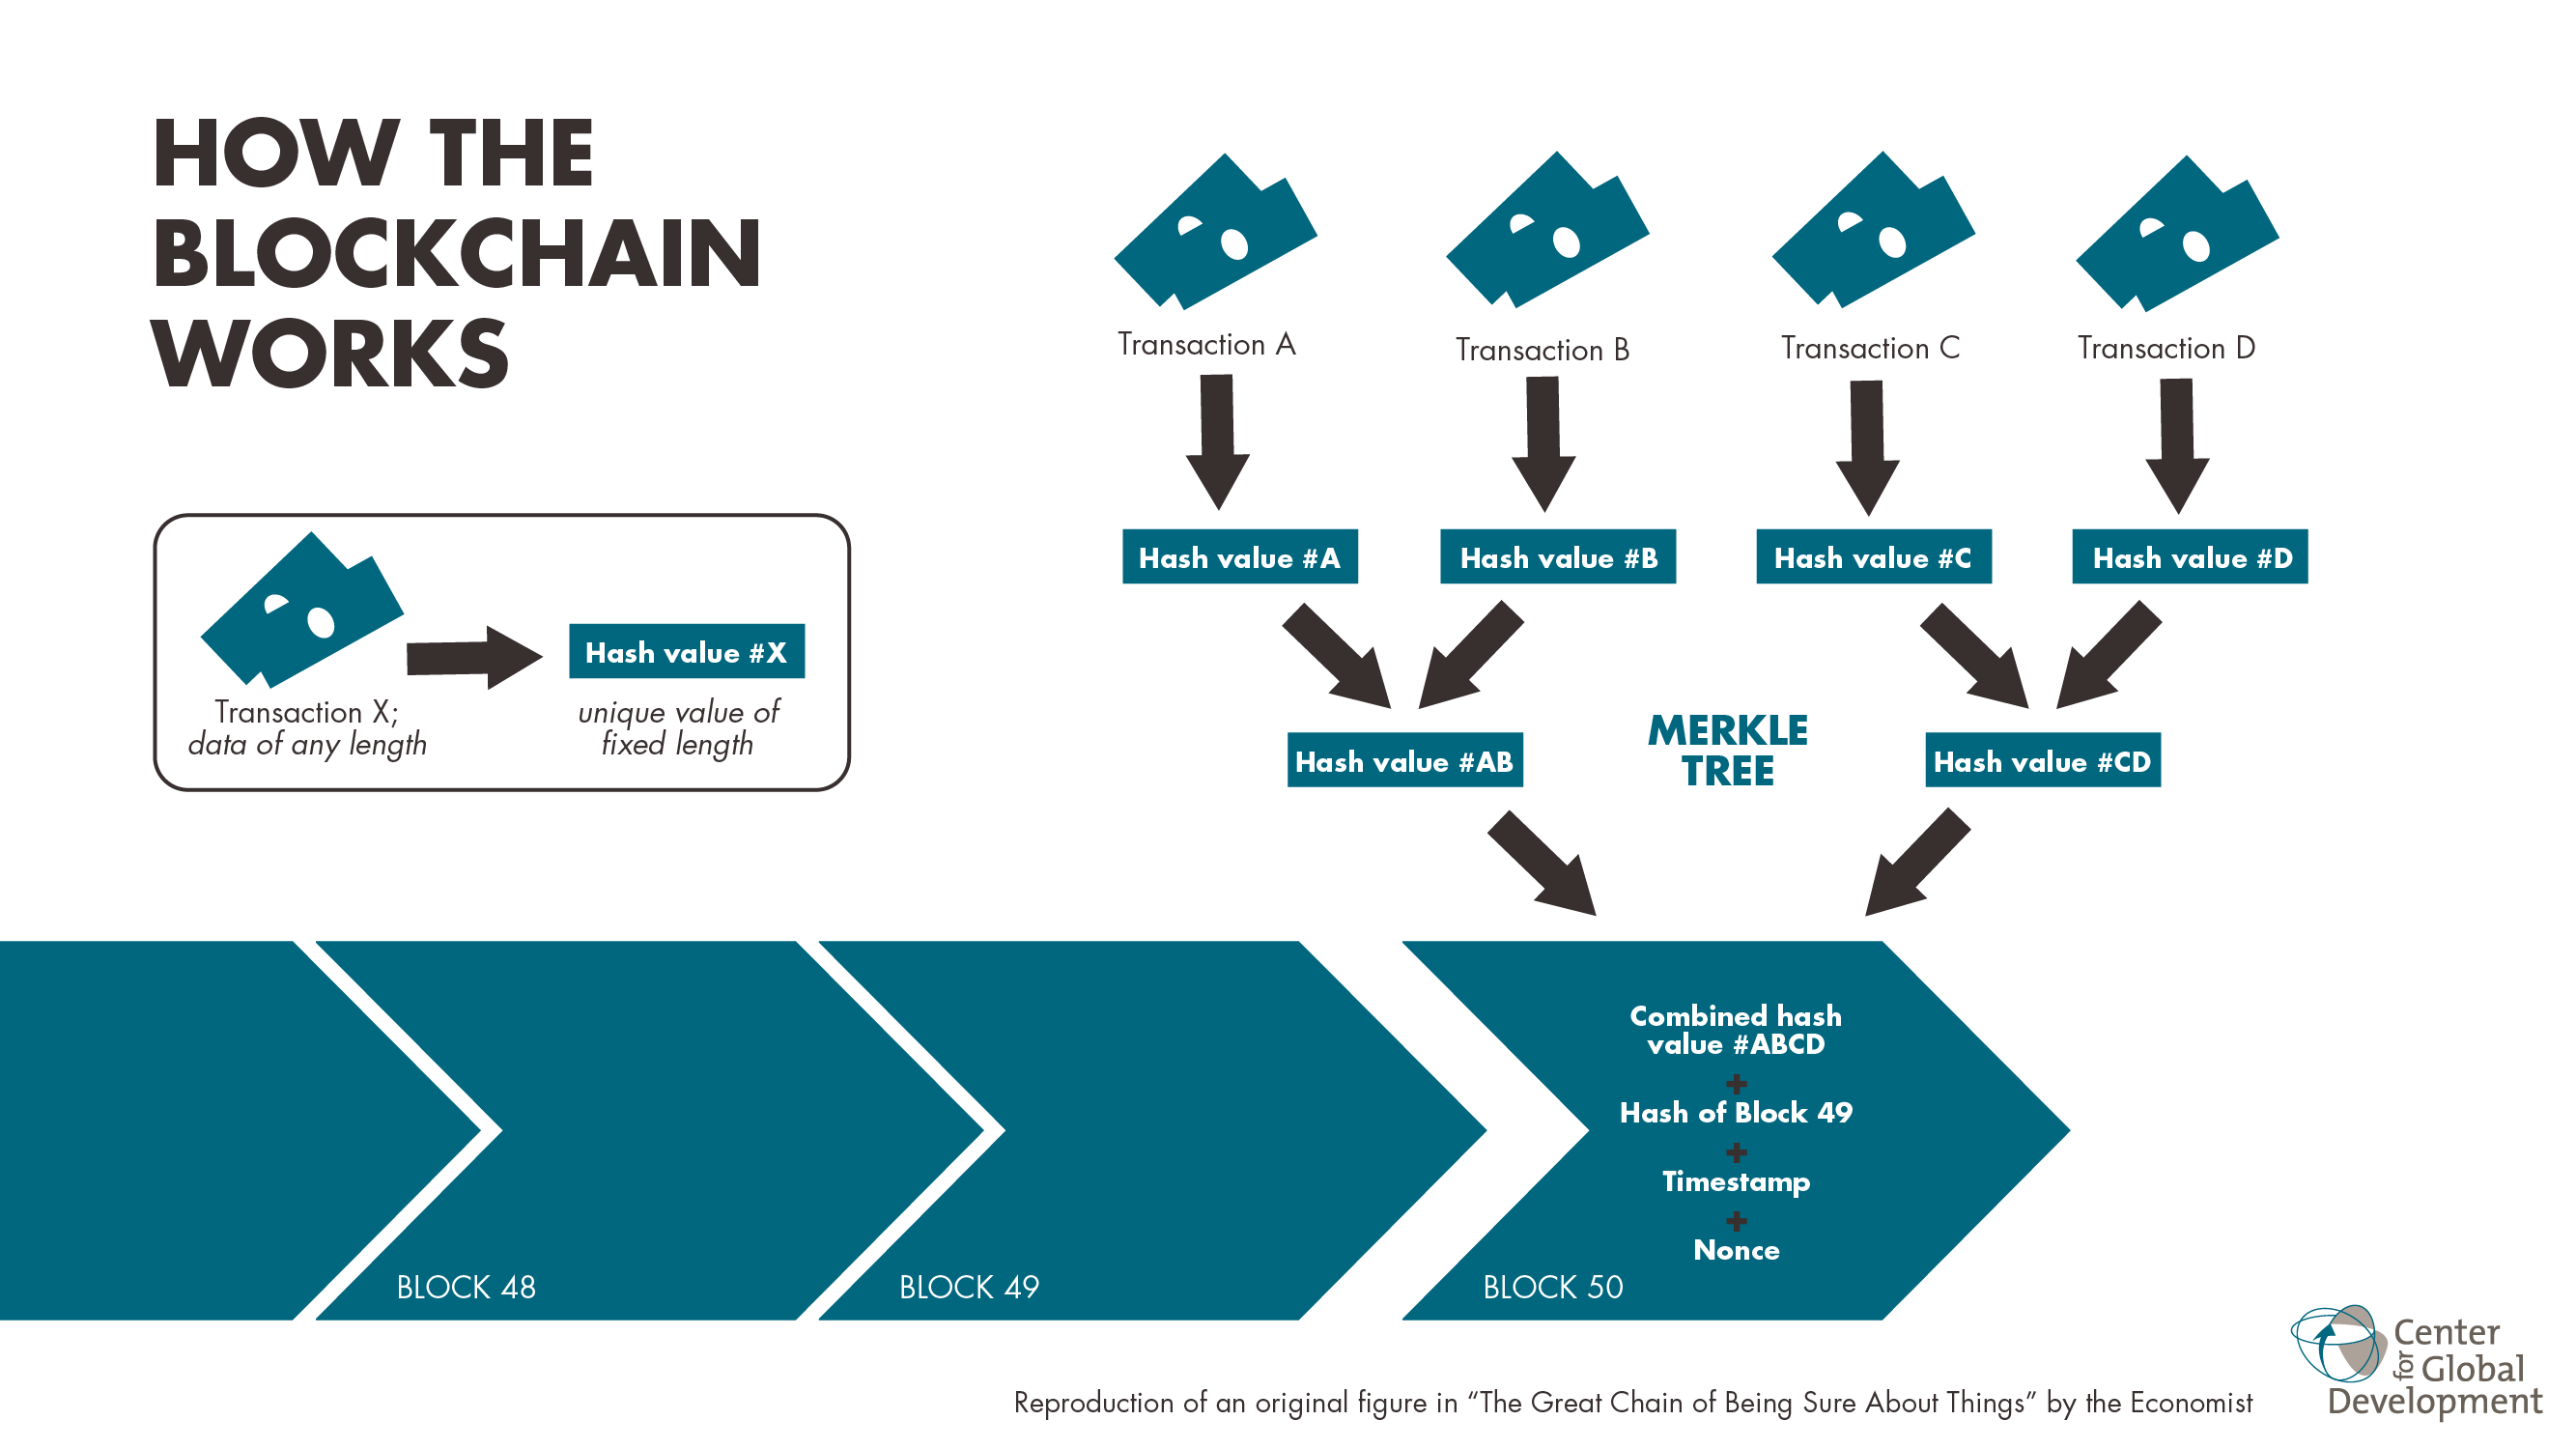
\includegraphics[scale=0.35]{media/Blockchain_workflow.png}
\caption{Representation of a blockchain's structure}
\label{fig:blockchain_workflow}
\end{figure}

\subsection{Immutability}
    This hash thus guarantees that the blocks are linked to each other, but it also guarantees the integrity of the block chain. If one block is altered, the hash on the block that follows it stops matching the block's. If we really wanted to change something on this  first block, we would have to alter the hash on the following block to match. But then, that second block would also have been altered, and we would have to change the hash on the third block to match, and so on. This means that the blockchain is immutable, as it is not possible to alter a single block without manually altering all the others. 
    
\subsection{Consensus}
    The blockchain and its data exists only in a \textbf{peer-to-peer network}, and as such, it is stored and extended by the nodes of the network, which form a topology between them. The nodes are machines that have the core code of the blockchain system and which receive and share among themselves the incoming information, in the form of blocks, validating it according to the established rule set. All the nodes, if they are not malicious and actively attempting to change the contents of the chain, contain the same blockchain structure and information, as they all agree on its contents through a consensus algorithm. 
    
     Some nodes are open to the internet and the world, thus receiving information from outside the peer-to-peer network and disseminating it to the rest of the network's nodes. A subset of the nodes, called miners, will then gather the circulating information from the peer-to-peer network (by receiving transactions from the nodes they are connected to), and form blocks of information, which they try adding to the blockchain. Obviously, it is impossible for all the nodes to add their blocks at the same time, as each of them would then have a different version of the blockchain and they would get desynchronized. And so, the nodes must reach a consensus as to which block gets added next to the blockchain. For this very reason, the code of the blockchain must have both a consensus algorithm and also a block validation algorithm.
     
     In public blockchains, the mining nodes do all the hard work, and they usually need some incentive to do so. Cryptocurrencies are virtual currencies that only exist on the blockchain they belong to, and they allow for a new monetary system to come into life. These currencies play an important role in blockchain, since they allow for miners to be rewarded. Without them, public blockchains would probably not work as well, which is why there are so many alternative currencies popping up, with the advent of this technology. 
     
     Of course, this is just one of many ways to make a blockchain move forward successfully, and other types of consensus algorithms have been idealized, though most of the consensus algorithms in public blockchains will use cryptocurrencies as the prime incentive.
    
    
\subsection{Private, Public and Hybrid Blockchains}

    Blockchain, traditionally, is of public nature. But, as many institutions grew aware of the possible benefits of this technology, they started investing in it, and so appeared the private blockchains and the semi-private or consortium blockchains.
    
    \paragraph{Public Blockchains} When a blockchain is public, it is accessible to any user. Anyone is able to both read and validate information from it, as well as contribute to its extension by participating in the consensus process. They are secured by the economic incentives that are given to the miners, in the form of cryptocurrency tokens. These blockchains can be  considered fully decentralized and have no access control. Every user is at the same level.
    
    \paragraph{Private Blockchains} These are usually owned by some organization and have access control, restricting write access to certain peers inside the organization. Read access might be restricted or not, according to the organization's goals. These blockchains, unlike public ones, might not require cryptocurrency or incentives, as the maintenance of the blockchain is done by the organization who owns it, and so they have all the interest in having nodes that can run the consensus process. In the end, this is a more centralized version of the blockchain, as the nodes are concentrated under the ownership of the organization. This also gives the advantage that alterations to the blockchain are easier to achieve, if so is desired (though it subtracts from the actual meaning and concept of an immutable blockchain). It is usually more efficient than public blockchains, being able of achieving a higher number of transactions processed per second.
    
    \paragraph{Consortium blockchains} They are a kind of hybrid blockchain, though closer to a private blockchain. They are controlled by many different organizations, and the consensus process is handled by pre-selected nodes from the organizations. This consensus might involve, for example, at least a certain percentage of the nodes agreeing on something (e.g.: if there are 15 fixed nodes, require at least 10 to sign the block). The permissions to read might be public or otherwise permissioned, and as such, this can also be considered a partially decentralized blockchain.
    % TODO: INCLUDE QUOTE
   % “So far there has been little emphasis on the distinction between consortium blockchains and fully private blockchains, although it is important: the former provides a hybrid between the ‘low-trust’ provided by public blockchains and the ‘single highly-trusted entity’ model of private blockchains, whereas the latter can be more accurately described as a traditional centralized system with a degree of cryptographic auditability attached.”[2] 

%--> Hyperledger composer leans more towards the consortium permissioned blockchain type
    \subsection{Types of Consensus Mechanisms and Algorithms}
    
     The most commonly used consensus algorithm is \textbf{Proof of Work (PoW)}, though there are others, like the most used alternatives, \textbf{Proof of Stake (PoS)}, and \textbf{Proof of Activity (PoA)}. We showcase some of the algorithms in table %TODO: PUT REFERENCE 2.1.
    
%%%%%%%%%%% TABLE

%TODO: FIX THIS

% Please add the following required packages to your document preamble:
% \usepackage[normalem]{ulem}
% \useunder{\uline}{\ul}{}
\begin{table}[]
\centering
\caption{My caption}
\label{my-label}
\begin{tabular}{|l|l|l|}
\hline
Type                                                                       & Overview                                                                                                                                                                                                                                                                                                                                                                                                                                                                                                                                                                                                     & Better Used In                                                                           \\ \hline
Proof of Work (PoW)                                                        & \begin{tabular}[c]{@{}l@{}}In short, PoW works by making the nodes spend \\ computational power until they can find out a hash \\ that satisfies a certain rule, for a certain block. When \\ a node finds this hash, it is allowed to extend the \\ blockchain with that block. The node transmits the \\ new blockchain to all the other nodes. It is assumed \\ that the longed valid chain (where all blocks have \\ valid mininghashes and valid contents) held by any \\ block is the correct one. Additionally, the creator of \\ a block includes a reward for themselves in the block.\end{tabular} & \begin{tabular}[c]{@{}l@{}}Public Blockchains\\ (Bitcoin, alt coins)\end{tabular}        \\ \hline
Proof of Stake (PoS)                                                       & \begin{tabular}[c]{@{}l@{}}In PoS, the "miners" stake their cryptocurrency \\ tokens as a bet, on which block they want to \\ include in the blockchain. By doing so, they \\ actively have a chance to mint that block \\ proportional to the number of tokens they \\ stake. This makes it so that any participant of the \\ network has in its best interest to be honest. The \\ higher their stake, the more invested in the \\ network they are. PoS is less wasteful than PoW, \\ which consumes a lot of energy in computational \\ power.\end{tabular}                                              & \begin{tabular}[c]{@{}l@{}}Public Blockchains,\\ Consortium \\ Blockchains\end{tabular}  \\ \hline
\begin{tabular}[c]{@{}l@{}}Proof of Authority\\ (PoA)\end{tabular}         & \begin{tabular}[c]{@{}l@{}}The transactions are validated, aggregated into blocks \\ and put into the blockchain by approved known nodes,\\  which act like "admins" and are the source of truth \\ for the system. This is a more centralized kind of \\ consensus.\end{tabular}                                                                                                                                                                                                                                                                                                                            & Private Blockchains                                                                      \\ \hline
\begin{tabular}[c]{@{}l@{}}Proof of Elapsed\\ Time (PoET)\end{tabular}     & \begin{tabular}[c]{@{}l@{}}Every participant in the network is assigned a random\\  amount of time to wait, and the first participant to \\ finish waiting gets to commit the next block.\end{tabular}                                                                                                                                                                                                                                                                                                                                                                                                       & \begin{tabular}[c]{@{}l@{}}Private Blockchains,\\ Consortium \\ Blockchains\end{tabular} \\ \hline
\begin{tabular}[c]{@{}l@{}}Byzantine Fault \\ Tolerance (BFT)\end{tabular} & \begin{tabular}[c]{@{}l@{}}There are many algorithms for this kind of consensus.\\ One is Practical BFT (PBFT), with pre-selected nodes \\ selecting and ordering the transactions.\end{tabular}                                                                                                                                                                                                                                                                                                                                                                                                             & \begin{tabular}[c]{@{}l@{}}Private Blockchains,\\ Consortium \\ Blockchains\end{tabular} \\ \hline
\end{tabular}
\end{table}



%%%%%%%%%%% TABLE END


 .
    
    \subsection{Transparency}
   The blockchain is not only available to the mining nodes in the network. Though they are the ones who actively interact with the chain in order to make it grow, if the chain is public, anyone can view the records and verify the authenticity of the data. This is the property of transparency. In private or permissioned blockchains, it might happen that only certain actors have access to certain records, according to the access control rules set by the organization or set of organizations that manage it. This is done with the help of sets of asymmetric key pairs and a public key infrastructure.
    
% Talk about merkle tree - is it necessary?


%\section{Security Features}
%In a blockchain, security is a multi-faceted aspect. It depends heavily on cryptography, especially hashing and public key cryptography. But it also depends on a blockchain's characteristics and set values, such as the average block time.
%\paragraph{Hashing}
%\paragraph{Public Key Cryptography}
%\paragraph{Other aspects and concerns}

\section{Applications}

    In general, blockchains are applied in different ways, from public ledgers to private, in a continuum, according to the specific needs. Many of them even apply the concept of smart contracts. Vitalik himself suggested some possible applications of Ethereum, and many more have been idealized, with some even being successfully applied. Here are some examples of areas where the benefits of introducing blockchain have been studied.
    
%\todo{It could make sense to mention, for each of the aread below, the key properties of a blockchain that it expectedly benefits from.}
% In the frameworks chapter, it is mentioned a bit better than here

    \begin{itemize}
     \item Identity/Record Management - like in a notary, documents are validated and recorded.
     
     \item Insurance - Smart contracts, having to abide to certain rule with certainty, make for a perfect system for risk-management. Given that certain conditions are met, the insurance could be claimed, giving way to faster and less error-prone insurance processing.
     
     \item Health care - Health records easily accessible anywhere. This could be coupled with other applications, like using sensors and smart contracts to automatically monitor patient status.
     
     \item Distributed Cloud Storage - Instead of the traditional centralized cloud, distributed clouds could become a reality.
     
     \item Voting - Using blockchain, digital voting could become feasible. The greatest barrier to e-voting have been the concerns with security, and blockchain provides an anonymous and secure way to do it.
     
     \item Internet-of-Things (IoT) - Any object connected to the Internet can upload information, which can either be stored or processed on the blockchain. Devices with sensors, for instance, can be programmed to send their values to the blockchain, which can then be queried by others to check these values. There can even be pre-programmed smart contracts that have events based on what is happening and the information that is being sent by the devices.
	\end{itemize}

    \chapter{Blockchain Frameworks}
\label{chap:blockchain-frameworks}

%\minitoc \mtcskip \noindent
Not sure if this would have enough content to be a whole new chapter, it could probably be integrated in the previous one, we'll see.

\section{Ethereum}

With the purpose of building a blockchain that does more than just provide a currency system, the Ethereum project was developed and launched in 2014. A white paper, written by Vitalik Buterin was released explaining the concepts and inner-workings of this platform, and its popularity has been growing ever since. Citing Buterin's paper, Ethereum has the intent to \textit{"allow developers to create arbitrary consensus-based applications that have the
scalability, standardization, feature-completeness, ease of development and interoperability" } \cite{Buterin2014}.

\subsection{Smart Contracts}
In short, Ethereum is a blockchain platform that implements a Turing-complete programming language, allowing for the existence of code stored in the form of "contracts". This allows for the practical existence of Smart Contracts, a concept first proposed by Nick Szabo in 1996 \cite{szabo1996smart}. According to Szabo, \textit{"A smart contract is a set of promises, specified in digital form, including protocols within which the parties perform on these promises."} 

So, at a more superficial level, a smart contract is just code, a structure that follows pre-specified rules, in order to move around assets, such as cryptocurrency tokens, and change its state. It reacts according to the interactions it has with the other elements of the blockchain, which, in a crude manner, can be either people or other contracts. In other words, Ethereum moves beyond the realm of currency and opens up the possiblity for decentralized applications to be ran directly on the blockchain. 

%In general, there are
%two types of accounts: externally owned accounts, controlled by private keys, and contract accounts, controlled
%by their contract code. An externally owned account has no code, and one can send messages from an
%externally owned account by creating and signing a transaction;
%in a contract account, every time the
%contract account receives a message its code activates, allowing it to read and write to internal storage and
%send other messages or create contracts in turn.

\subsection{Currency}

The interesting aspect of Ethereum, however, is that the code from these applications or contracts is executed by the peer-to-peer network nodes, making Ethereum a globally available computer. Of course, with computational power comes a price. Each time a function from a contract is called, someone's computer, a mining node, is doing all the computations, and for each line of code, an agreed fee must be paid. As such, Ethereum has its own cryptocurrency, by the name of Ether, and which is essential to fuel the network.

\subsection{Consensus}

At the moment, Ethereum is still using PoW as the consensus protocol, in a similar fashion to Bitcoin. There are projects currently trying to move Ethereum to PoS, such as Casper \cite{Buterin2017}. PoS is a consensus protocol with a different paradigm, in which the block mining process is roughly based on trust, on the fact that the miner has a certain stake or investment (like cryptocurrency) in the network, and so it is in their best benefit to be an honest node. 

The benefit of PoS over PoW is that there isn't as much waste of computational power as in PoW. In PoW, miners have to intensively search for a target number, which allows them to claim the block as their own. This serves no other scientific or practical purpose other than making the mining process hard, and, as soon as a node successfuly mines a block, all the energy used  by all the other mining nodes that were in this process basically goes to waste \cite{Buterin2013}. There are other concerns that make a PoS system like Casper a better option as well, such as performance concerns. 

\subsection{Performance and Scalability}

\paragraph{Issues} 
- Check original scalability issues from white paper

Ever since its conception, there has been concern as to whether Ethereum's throughput and latency are enough to handle a large amount of applications running at once, and if it will be scalable in the future. The recent launch of an application by the name of CryptoKitties disrupted Ethereum, congesting the main network and slowing down the speed of transactions, again raising concern over Ethereum's performance.

These concerns are also very much valid for the case of supply chains. If Ethereum were to be integrated with a supply chain, one of the most important factors to take into account would be the performance and scalability of the system. It is important to note, though, that private and public blockchains have different performances as well as different scalability concerns. Furthermore, certain values that affect the performance (such as the block time) also have an affect on security. This means that there is a bootstrap effect between security, performance and scalability.

In a public chain, security is a much bigger concern, as there are many different kinds of attacks, and the blockchain's values are balanced in a way that tries to prevent these. Such values can easily be adjusted in a private chain, in ways they can't in a public chain, where they would cause forks, clog the chain or raise security issues. 

The performance of blockchains such as Ethereum is usually measured by the average throughput, which is the number of processed transactions per second (TPS). This depends a lot on two main factors:
\begin{itemize}
\item The block size - in Ethereum, the block size is not a fixed value; rather, it has a "gas" limit; each transaction put into the block spends some gas, and when the gas reaches the limit for that block, the block is full;
\item The average time to publish a block - block interval; in Bitcoin, this was a fixed 10 minute time, but in Ethereum, the average time is around 15 seconds; this is directly related to the latency, the time a transaction takes to be integrated into the blockchain;
\end{itemize}

The fact that both transactions and block can vary in their size makes it hard to theoretically pinpoint what the performance of an Ethereum network is. In practice, though, and according to recent studies and statistics gathered, the throughput of the main Ethereum network is around 15 TPS.

\paragraph{Practical values}
In practice, it can handle

 Every node validates all the transactions: this is wasteful

\paragraph{Casper}
It allows the throughput of the network to increase.

The block time is able to be lowered because validators aren't burning cash on electricity to mine

\paragraph{Sharding}
- sharding

\paragraph{Plasma}
- Scalability (check recent paper from Vitalik) + plasma (check from Joseph Poon)

- Public blockchain and private would scale differently
\break

%EXCERPT FROM ARTICLE-THESIS, to take some info out:
%"Probably the biggest scalability issues with Ethereum are that every node has to process all
%transactions and has to store the entire state of every account balance, contract code and
%storage, etc. Although this provides a large amount of security, but greatly limits scalability
%to the point that a blockchain cannot process more transactions than a single node. One
%would think that a network with thousands of nodes should be able to have more throughput
%than a single node, but this is not the case in Ethereum or in public blockchain networks in
%general.
%A possible solution for this problem is to create a new mechanism where only a small subset
%of nodes has to verify a subset of transactions. As long as there are sufficient many nodes
%verifying each transaction, the system will still be secure, but also allow for the system to
%process transactions in parallel. This techniques is called sharding. The basic idea behind
%sharding is by dividing the global state of accounts, both external and contract accounts,
%in smaller chunks known as a shard. In simpler forms of sharding, each shard also has its
own transaction history, and the effects of transaction in some shard K are limited to the
state of shard K. However, transactions across two shards can be achieved with a ”debit”
and ”credit” kind of transactions. For example a transfer of money, where money is moved
from shard K to shard L by first creating a ”debit” transaction that destroys coins in shard
K, and then creating a ”credit” transaction that creates coin in shard L, pointing to a receipt
created by the debit transaction as proof that the credit is legitimate. In more complex
forms of sharding, transactions may in some cases affect other shards as well and may also
synchronously ask for data from the state of multiple shards. Each shard gets its own set of
validators, and these validators will not need to validate all shards[35]."

\subsection{Usability}
- Explain that, though there is a main ethereum network, it can also be deployed privately

- Examples of companies that Ethereum, either in the public chain, or in a private one

\subsection{Ethereum Applicability to Supply Chain}
Maybe this subsection is already what is described in the sections that follow, such as section 3.5 Applications and so on. Especially in section 3.5, I should explain better how the Applications of Ethereum (section 3.4.4), can be applied in general
- Talk about Eth possible applicability, because of the fact it might be expensive;

\section{Hyperledger}

\section{Corda}

\section{Comparison}

    \chapter{Blockchain in the Industry}
\label{chap:blockchain-applicability}

\minitoc \mtcskip \noindent

This chapter presents an overview of how the blockchain might apply to the industry in general and supply chain in particular. It goes on to describe the general advantages of using blockchain, with a focus on how it might positively affect SCM, as well as the disadvantages and challenges the integration of blockchain might face. Some applications that are already trying to merge the concepts of blockchain and Supply Chain are presented. Finally, an overview of some design alternatives are given, which will be the basis for the design analysis  and decisions later on. 

The purpose of this chapter is, given all the information already presented, to present some topics that might unify the topics of blockchain and supply chain into one, to ascertain if they are a good fit.

\section{Advantages of Blockchain in Supply Chain}

Some of the advantages blockchain would bring to supply chain, over other solutions:

\begin{itemize}
\item \textbf{Less error prone}: reduction in errors on manual data entries, especially when combined with IoT and other automated processes; any other kind of error that manages to find its way into the system is easily traceable.
\item \textbf{Enhanced security of transactions}: not only is the ledger immutable, attempts at fraud are easily detected.
\item \textbf{Improved tracking}: the ledger is easy to analyze and delivers the results really fast, making it possible to know the status of any order or asset at any time.
\item \textbf{Improved consumer trust}: blockchain could allow users to check the provenance of their products, developing a relationship of trust with the suppliers.
\item \textbf{Reduced costs}: \textbf{reduced governance costs} for exchanging info and etc, allowing for higher efficiency and faster times at processing the information (enhancing cost effectiveness); \textbf{reduced internal management costs}, increasing efficiency and sustaining competitiveness; \textbf{reduced product or service costs}, creating competitive advantage and barriers to competition, reduced supply chain lead times and increased flexibility in supply chain design. %[21].
\item \textbf{Internal supply chain trust}: It is important that the elements of a supply chain trust the information that comes and goes from each other, and blockchain allows this to happen.

\end{itemize}

%[CITE DSC ARTICLE HERE?]

This last point is one of the most important aspects, which is often overlooked in favor of other more obvious functionalities.

As described by Panayides \cite{Panayides2009}, co-operation and trust are the key in improving supply chain performance and innovativeness, increasing the quality and leading to benefits for all parties involved. Similarly, Yeung \cite{Yeung2009} managed to find a relation between trust and a higher supply chain integration. In the context of supply chains, trust might be defined as not only loyalty, but also reliability. This last aspect is very important, because it measures just how much you can expect from your partners in a supply chain. And when you need information quickly, trust in the form of reliability is a very important asset to have.

%\todo{fcorreia: "trust" can mean several things. 2hat does it mean to "trust" information? is it that elements of a supply chain don't trust that the information comes from the source that they think it does? is it that they don't trust that the network doesn't drop any information? or is it that they don't trust that the *people* upstream in the supply chain record all the information accurately? My best guess would be that this last question is the relevant one in the context of supply chains, but I don't think that a blockchain would help that much here. WDYT?}
%It's all of them, actually... If you're a business, you only trust your own information and you only rely on yourself, you don't expect others to be 100% cooperative and fully functioning all the time. 

In this sense, if the blockchain technology manages to improve the information flow in a supply chain, while maintaining security and trust between parties (at least at a technical level), then it follows that, just as concluded by Panayides and Yeung, the supply chain itself will have an improvement in performance, since the parties involved don't have to worry as much about these aspects or any power struggles. Therefore, \textbf{trust seems to be a key factor in building an efficient and effective supply chain}.

\section{Challenges of Blockchain Application to Supply Chain}

The reverse side of the coin is that Blockchain is not always the amazing solution that is prophesied. Blockchain itself is a topic in research and, while some of its applications and advantages are quite obvious, many of its disadvantages are overlooked, and these might be crucial when making the decision to apply blockchain to a supply chain.
%Check image from the other article
%Other article talking about the throughput and latency trade-off.
\subsection{Technical Limitations and Scalability Concerns}
The technical limitations include, but are not limited to: throughput, latency, size and bandwidth and security.

\begin{itemize}
\item \textbf{Throughput}: Current blockchain technologies, even in private deployments, such as Hyperledger, have a high throughput, but not as high as certain centralized systems. This is one of the main concerns in supply chain, that a blockchain can't process the information quite as fast as the current systems, which could lead to a decrease in performance and further delays. As in any distributed system, though, the decrease in speed is often the price to pay for decentralization in supply chain. Ultimately, while the flow of information inside one specific company might be lower than before, the flow between different companies, which were previously not integrated, might actually be much faster than before. It is not fair to compare the speed of a centralized system with the speed of a distributed ledger, since the latter offers more functionality and disperses the information further where the former couldn't. A slower dispersion of information globally, through various entities, is, in this case, preferred to a fast dispersion only locally, through an organization's system or its closest associates.
\item \textbf{Latency}: Similarly to throughput, and related to it as well, the latency of a transaction is something to take into account. With some blockchain deployments, like Bitcoin, each transaction might take a long time to validate, and this time might depend on the fees paid as well. This is mitigated by permissioned platforms such as Hyperledger, which have low latency, even in the presence of a high number of transactions, and possess no currency or fees to worry about.
\item \textbf{Size}: The more transactions are processed and information stored in the blockchain, the bigger it actually grows. In the current context, if we were to deploy a global blockchain for all the supply chains, it would probably grow way too large in a small amount of time, which would not be sustainable in the long run. In a more limited scope, however, it would probably not be as big of a problem. There is also a lot of research in the optimization of blockchain size.
\item \textbf{Security}: One concern for blockchains in general is how security is handled. This issue is more important in the case of public blockchains with PoW consensus. In the case of supply chains, there are many alternatives, and possibly having a public PoW blockchain is not the optimal one, so this is not the main security aspect to worry about. There is, however, another aspect to take into account, which is the fact that the hash functions being used at the moment might be broken in some years. If this were to happen, the immutability property of a blockchain would be broken and any prospects of proving the provenance of products or their traceability would lose their groundwork.
\end{itemize}

\subsection{Lack of Interoperability Standards}
Provided that there is a way to share information, companies each have their own means of inserting information into their systems, in whichever format they want, as long as the correct pieces of information are there. Other companies which might want to access this information might have a difficult time understanding just what to look for and where to look for it. 

This is the first part of the problem, the lack of standards by which companies should abide to, if they want to form some common ground by which they can cooperate and understand each other's information. 

The second part of the problem deals, in a more technical way, with the lack of interoperability in the system's themselves. Many ERPs are operated under closed environments, with information often being manually entered into the system, and no APIs for external systems to connect to.

\section{Similar existing applications}
Some projects which try to fit blockchain as a solution for improving SCM have already emerged, or are in being worked on. This section explores some of these applications.

\subsection{IBM and Maersk's Demo}
IBM, together with Maersk, just recently launched an innovative project which aims to create an open platform, using Hyperledger, for information sharing on a large scale \cite{A.P.MOLLER-MAERSK}.

It is an open platform, which features a shipping information pipeline and paperless trade. It deals mostly with the transportation of goods and automating all the processes associated with it.

%\todo{fcorreia: nothing more to say about this? would be interesting to know in which way it compares with your goals and with the other similar applications}
%It was just announced and they have no articles explaining it yet...

\subsection{CargoX}
%\todo{fcorreia: something that would be great to have in the document (but probably not here) is an analysis of relevant concepts within the domain of supply chain management; possibly including a domain model.}
CargoX delivers a solution for making the Bill of Lading (B/L) documents digital.  To give some context: in a supply chain, many times, the products are delivered by cargo ships, inside containers. The B/L document has the same value as the value of the goods that are declared on it, serving the following functions:
\begin{itemize}
\item It is a receipt that acknowledges the loading of the products.
\item It contains the terms of the contract of carriage.
\item It is a title to the goods it declares.
\end{itemize}
These characteristics make it an extremely valuable document, which must be transferred from the carrier to the company acquiring the products in a safe way. Losing this document would mean losing the rights to all the goods in the shipment, as well as losing the proof that they were even shipped in the first place.

CargoX uses Ethereum's smart contracts to put these paper documents into the blockchain. It has a built in token system that allows to exchange the document's ownership immediately after payment \cite{CargoX2017}.

\subsection{Eximchain}
Eximchain is an all-round solution, which acts as a ledger, recording historical data and transactions, as an inventory management tool and also provides financial applications, by means of smart contracts. It was developed using a fork of Ethereum, Quorum, which is a permissioned version of Ethereum, focused on enterprise use, which means Eximchain runs on its own network \cite{Huertas2017}.

\subsection{OriginTrail}
Like CargoX, origintrail operates on the Ethereum network, and has its own tokens. It synchronizes all supply chain data in the platform, and uses these tokens as an incentive.

Its objective is to ensure traceability of the products as they move from supplier to retailer, all while ensuring the data is not tampered with. The tokens serve as a way to exchange data ownership, as well as to make reviews on a reputation system. \cite{Rakic2017}

\section{Designing a Blockchain-based Supply Chain}
%CHECK https://modum.io/system/

Blockchain is not always a one-size-fits-all solution, and its use must be carefully tailored to the application in question and to the specific requirements. This section describes some important points of focus to have in mind when making decisions for the design of a blockchain based supply chain.

\subsection{Integration Models}
\paragraph{Point-to-point} Business-to-Business (B2B) Data Interchange - The integration must be designed between each two specific endpoints. Each new connection must be modeled separately. In a large scale, this does not work very well, it is a model that only works under specific cases and requirements, since it requires a customized integration.

\paragraph{One-to-many entities} Hub B2B - A company can develop a connection endpoint to which other companies can connect, as long as they follow the hub's communication standards or use its API. This way, a  single company can establish connections with multiple intermediaries.

\paragraph{Many-to-many entities} Cloud B2B - This model encompasses full integration, where the information can flow freely between businesses. This is the ultimate goal of a public blockchain, but it would require companies the development of interoperability standards, which are, at the moment, lacking. Otherwise, it is the most cost-effect model and the one which can bring about the most benefits as well, given that the companies can develop their services to be integrated with the blockchain.

\subsection{Key Implementation Components and Features}
As seen in the previously mentioned projects, like CargoX, Eximchain and OriginTrail, each of them followed their own purpose and goals, and each of them has a different set of features that allows them to achieve these goals. Similarly, these are some of the key components that a blockchain possesses, and the respective features that must be decided upon:

\paragraph{Information Storage}
The most basic and important feature of a blockchain is the ability to save data, which is then considered immutable, as well as registering any important events. As such, information storage is a must in supply chain. It also makes possible Inventory Management possible (though it's implementation is out of the blockchain's scope), traceability and provenance of products.
      
\paragraph{Ledger and Transactions}
Similarly, allowing for transactions and their recording onto the chain might be important, especially in what accounts for payments between businesses.
  
\paragraph{Smart Contracts}
Finally, smart contracts have the potential to be an important part of SCM. In the applications we described, smart contracts were used to transfer ownership of either data or products through tokens. This is just one of the many possible uses. Other smart contract uses include tracking items by their location or condition, automatically updating the status on the blockchain and reacting to any important events by notifying the organization responsible for the items. Another possible functionality is the automation of payments upon delivery. In the end, smart contracts allow for virtually any application, since they are code, programs being run on the blockchain, and so, they are one of the components of blockchain with the most potential for new and innovative features to be developed upon.
        
%\todo{fcorreia: Something that could be fun to have in this section is a diagram depicting the different concerns that you have to consider and how these different concerns affect each other. For an example, take a look at the diagram in page 3 of this paper: \url{http://blog.invisivel.net/wp-content/papercite-data/pdf/ferreira_core_2010.pdf}}



	%\chapter{Applied designs for a blockchain driven supply chain}
\label{chap:problem}
% RESEARCH PROBLEMS

%\minitoc \mtcskip \noindent

Here, we talk concretely of the problem we will be researching. What will we be trying to figure out, to later implement? In this case, it is the designs for the blockchain

\section{Applied to the ledger}

\section{Applied to smart contracts}
	%\include{contribution1}
	%\include{contribution2}
	%\include{validation}
	\chapter{Conclusions}
\label{chap:conclusions}

\minitoc \mtcskip \noindent

%These conclusions are for PDIS; so they will close this delivery and may anticipate the expected results of the dissertation. Include the tasks and a Gantt diagram with the plan.
The dissertation focuses on finding out how applicable blockchain is to the supply chain industry and to SCM, and there are many variables to consider. Many companies have already started working on projects similar to what is trying to be accomplished here, though with a higher focus on financial benefits than on the research itself (many of the examples given were of companies using Ethereum and its tokens). These solutions have not yet been proved and are also taking their initial steps. The main focus of this dissertation is to develop a proof-of-concept that indeed blockchain can improve SCM in some form, and also give an insight on how this might be achieved. 

\section{Future Work}

The research for this dissertation is divided into six steps, described in Table \ref{table:gantt_chart} and illustrated by Figure \ref{fig:gantt_chart}. The research started with the literature review, which presents some important insights, frameworks as well as some important design aspects and decisions to take while developing a model for a blockchain-driven supply chain project.

These aspects will be taken into account for the next steps. First, adapting and creating a blockchain integration model, by making some decisions on the design and frameworks to be used. Then, a small integration project will be built based on this model.

In the final part of the project, its applicability and performance will be evaluated. The developed system itself is a proof-of-concept, which, already proves that such a concept might work, but it is important to measure how it fares against the traditional systems used in supply chain. This evaluation is done in two different parts: the first consists on evaluating functionality, and checking which functionalities are added or subtracted by using blockchain; the second part consists in using performance metrics to evaluate this dissertation's solution against the baseline of a traditional solution, like a centralized system. The metrics used to evaluate this include, but are not limited to:
\begin{itemize}
\item Throughput - processed transactions per second
\item Latency - average time to process a single transaction
\item Latency volatility - measure of the variety of latency
\item Security - qualitative evaluation that includes items such as immutability, denial of service resilience, trust and fraud protection, confidentiality and access control
\item Hardware requirements - how much hardware is needed, and how powerful
\item Scalability - number of nodes, transactions, users and how much the system can stretch these numbers
\end{itemize}

%\todo{fcorreia: do you have already any additional ideas about the baseline that you will be comparing to? it'd be great if you could provide a bit more detail about this; will it be a non-blockchain-based distributed system? (e.g., a microservice-based system, or a system based on a replicated datastore) Will it be simply a "normal" centralized system? Depending on the baseline that you choose the conclusions that you will be able to reach will be quite different}

Finally, the model might have to be recalibrated, taking into account the results gathered from these metrics. The values of the model might have to be changed iteratively, until a satisfying solution is achieved, if possible.

%%%%%%%%%%%%%%%%%%%%%%%% TABLE %%%%%%%%%%%%%%%%%%%%%%%%%%%%%%%%%

% Please add the following required packages to your document preamble:
% \usepackage[table,xcdraw]{xcolor}
% If you use beamer only pass "xcolor=table" option, i.e. \documentclass[xcolor=table]{beamer}
\begin{table}[]
\centering
\begin{tabular}{l|r|r|}
\cline{2-3}
                                                                                                  & \multicolumn{1}{l|}{{\color[HTML]{343434} \textbf{Starting}}} & \multicolumn{1}{l|}{{\color[HTML]{343434} \textbf{Ending}}} \\ \hline
\multicolumn{1}{|l|}{{\color[HTML]{343434} 1. Literature Review}}                                 & 1 Jan 2018                                                    & 9 Feb 2018                                                  \\ \hline
\multicolumn{1}{|l|}{{\color[HTML]{343434} 2. Decide on the features and design the model}}       & 10 Feb 2018                                                   & 5 Mar 2018                                                  \\ \hline
\multicolumn{1}{|l|}{{\color[HTML]{343434} 3. Create a small integration project}}                & 6 Mar 2018                                                    & 15 Apr 2018                                                 \\ \hline
\multicolumn{1}{|l|}{{\color[HTML]{343434} 4. Evaluate its applicability and performance}}        & 16 Apr 2018                                                   & 29 Apr 2018                                                 \\ \hline
\multicolumn{1}{|l|}{{\color[HTML]{343434} 5. Recalibrate the model's values, given the results}} & 30 Apr 2018                                                   & 14 May 2018                                                 \\ \hline
\multicolumn{1}{|l|}{{\color[HTML]{343434} 6. Finalize the dissertation document}}                & 15 May 2018                                                   & 22 Jun 2018                                                 \\ \hline
\end{tabular}
\caption{Work plan description for figure \ref{fig:gantt_chart}}
\label{table:gantt_chart}
\end{table}



%%%%%%%%%%%%%%%%%%%%%%%%%%%%%%%%%%%%%%%%%%%%%%%%%%%%%%%%%%%%%%%%
\begin{figure}[ht]
\centering
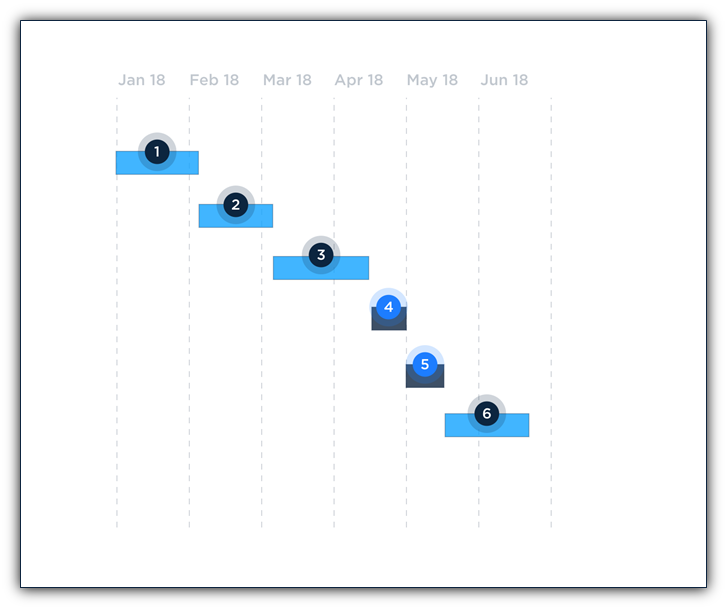
\includegraphics[scale=0.75]{media/gantt.png}
\caption{Research work plan}
\label{fig:gantt_chart}
\end{figure}

\section{Expected Results}
From this dissertation, it is expected that a proof-of-concept system with certain characteristics will emerge. The results will be analyzed to check if the system follows the parameters we are looking for.

For instance, it should be able to integrate information from various sources into a single place. This information should be available at any time, anywhere. It should be cryptographically secure, immutable, and easy and quick to share.

In the end, we need to analyze the results with the given metrics and ascertain whether there is a significant increase in performance and functionality that would justify using blockchain in a real supply chain.

%\todo{fcorreia: I'd expect to see here a list of contributions of your thesis. You do mention them, but a) I think they would be clearer to read as a list, b) you may be currently missing a few. I see at least 3 or 4, for example: a study of important design considerations for SCMSs, a study of important design considerations for blockchains, a prototype, an analysis of the benefits and liabilities of supporting a SCMS with a blockchain}

% pedro: I don't think a list is a good representation for the conclusion, especially when it is the ending of the document. And I don't know what other results to expect, I've written the ones we had discussed previously.




	\chapter*{Epilogue}
\addcontentsline{toc}{chapter}{Epilogue}  

Lorem ipsum


    \bookmarksetup{startatroot}
	\phantomsection
	\addcontentsline{toc}{part}{\appendixtocname}
	\appendixpage
	\appendix
		\chapter{Statistical Analysis Methodology}
\label{chap:appendix-a}


    % Please add the following required packages to your document preamble:
% \usepackage{multirow}
% \usepackage[normalem]{ulem}
% \useunder{\uline}{\ul}{}
\begin{table}[]
    \centering
    \caption{Data analysis metrics used in the survey results analysis}
    \label{annex:metrics}
    \resizebox{\textwidth}{!}{
    \begin{tabular}{l|l|l|}
    \cline{2-3}
                                                                                                                                 & Metrics                                                                & Meaning                                                                                                                                                                                                                                                                                                                                                                                                                                                                                                                                                                                                                     \\ \hline
    \multicolumn{1}{|l|}{\multirow{3}{*}{\begin{tabular}[c]{@{}l@{}}Measures of\\ Central Tendency \\ or Location\end{tabular}}} & \textbf{Mean}                                                          & \begin{tabular}[c]{@{}l@{}}The mean represents the most probable value. In this\\ survey, with the use of scales with a lower and upper\\ bounds, the mean has the roles of representing the\\ average value of agreement, importance and other\\ measures.Normally, when the skewness of a distribution\\ is high, the meaning of the mean may get distorted by\\ the existence of outlier values. However, since the scales\\ have a low range, with a lower and upper bound on the\\ answer values, this is not much of a concern. Therefore,\\ even in cases of skewness, the mean can be a useful metric.\end{tabular} \\ \cline{2-3} 
    \multicolumn{1}{|l|}{}                                                                                                       & \textbf{Median}                                                        & \begin{tabular}[c]{@{}l@{}}Value of the 50\% percentile, for numerical answers. Half\\ the answers are above this value and half are below,\\ pointing to a central tendency around this value. This is\\ a good metric to use, especially in skewed distributions\\ where there are outliers in the collected values, since the\\ meaning of the mean may get slightly distorted by the\\ outlier values.\end{tabular}                                                                                                                                                                                                     \\ \cline{2-3} 
    \multicolumn{1}{|l|}{}                                                                                                       & \textbf{Mode}                                                          & \begin{tabular}[c]{@{}l@{}}Most frequent response. Though it represents the most\\ popular answers, by itself the metric means nothing else,\\ as there might be answers almost as popular or not.\end{tabular}                                                                                                                                                                                                                                                                                                                                                                                                             \\ \hline
    \multicolumn{1}{|l|}{\multirow{2}{*}{\begin{tabular}[c]{@{}l@{}}Measures of Spread,\\ Scale or Dispersion\end{tabular}}}     & \textbf{\begin{tabular}[c]{@{}l@{}}Standard \\ Deviation\end{tabular}} & \begin{tabular}[c]{@{}l@{}}Quantifies the variation within the data set, by showing\\ how much the distribution spreads to either sides of the\\ center. A high value for the standard deviation means\\ that there are a lot of values away from the mean, from\\ which can be concluded that there is not a general\\ consensus on a certain answers.A low value means that\\ there is consensus, since all the values of the data set are\\ bundled more closely together.\end{tabular}                                                                                                                                  \\ \cline{2-3} 
    \multicolumn{1}{|l|}{}                                                                                                       & \textbf{Range}                                                         & \begin{tabular}[c]{@{}l@{}}Difference between highest and lowest value of the data set.\\ Together with the standard deviation, indicates the dispersion\\ of the value of the answers. A range of 0 means that a\\ question had the same value for all responses, for instance.\\ This metric ignores the frequency with which each answer\\ was given, that is why it must be coupled with the standard\\ deviation to be relevant.\end{tabular}                                                                                                                                                                          \\ \hline
    \multicolumn{1}{|l|}{\begin{tabular}[c]{@{}l@{}}Measures of\\ Skewness and\\ Kurtosis\end{tabular}}                          & \textbf{Skew}                                                          & \begin{tabular}[c]{@{}l@{}}This metric indicates the lack of symmetry in a distribution,\\ where the results bunch up in one side of the distribution.\\ For instance, negative skewness values indicate a skew to\\ the left: the values bunch up at the right end of the distribution\\ and the left tail is long, indicating there are outliers in the lower\\ values.\end{tabular}                                                                                                                                                                                                                                      \\ \hline
    \end{tabular}
    }
    \end{table}
		%\chapter{Composer Model Class Diagram}
\label{chap:appendix-b}

\begin{figure}[h]
    \centering
    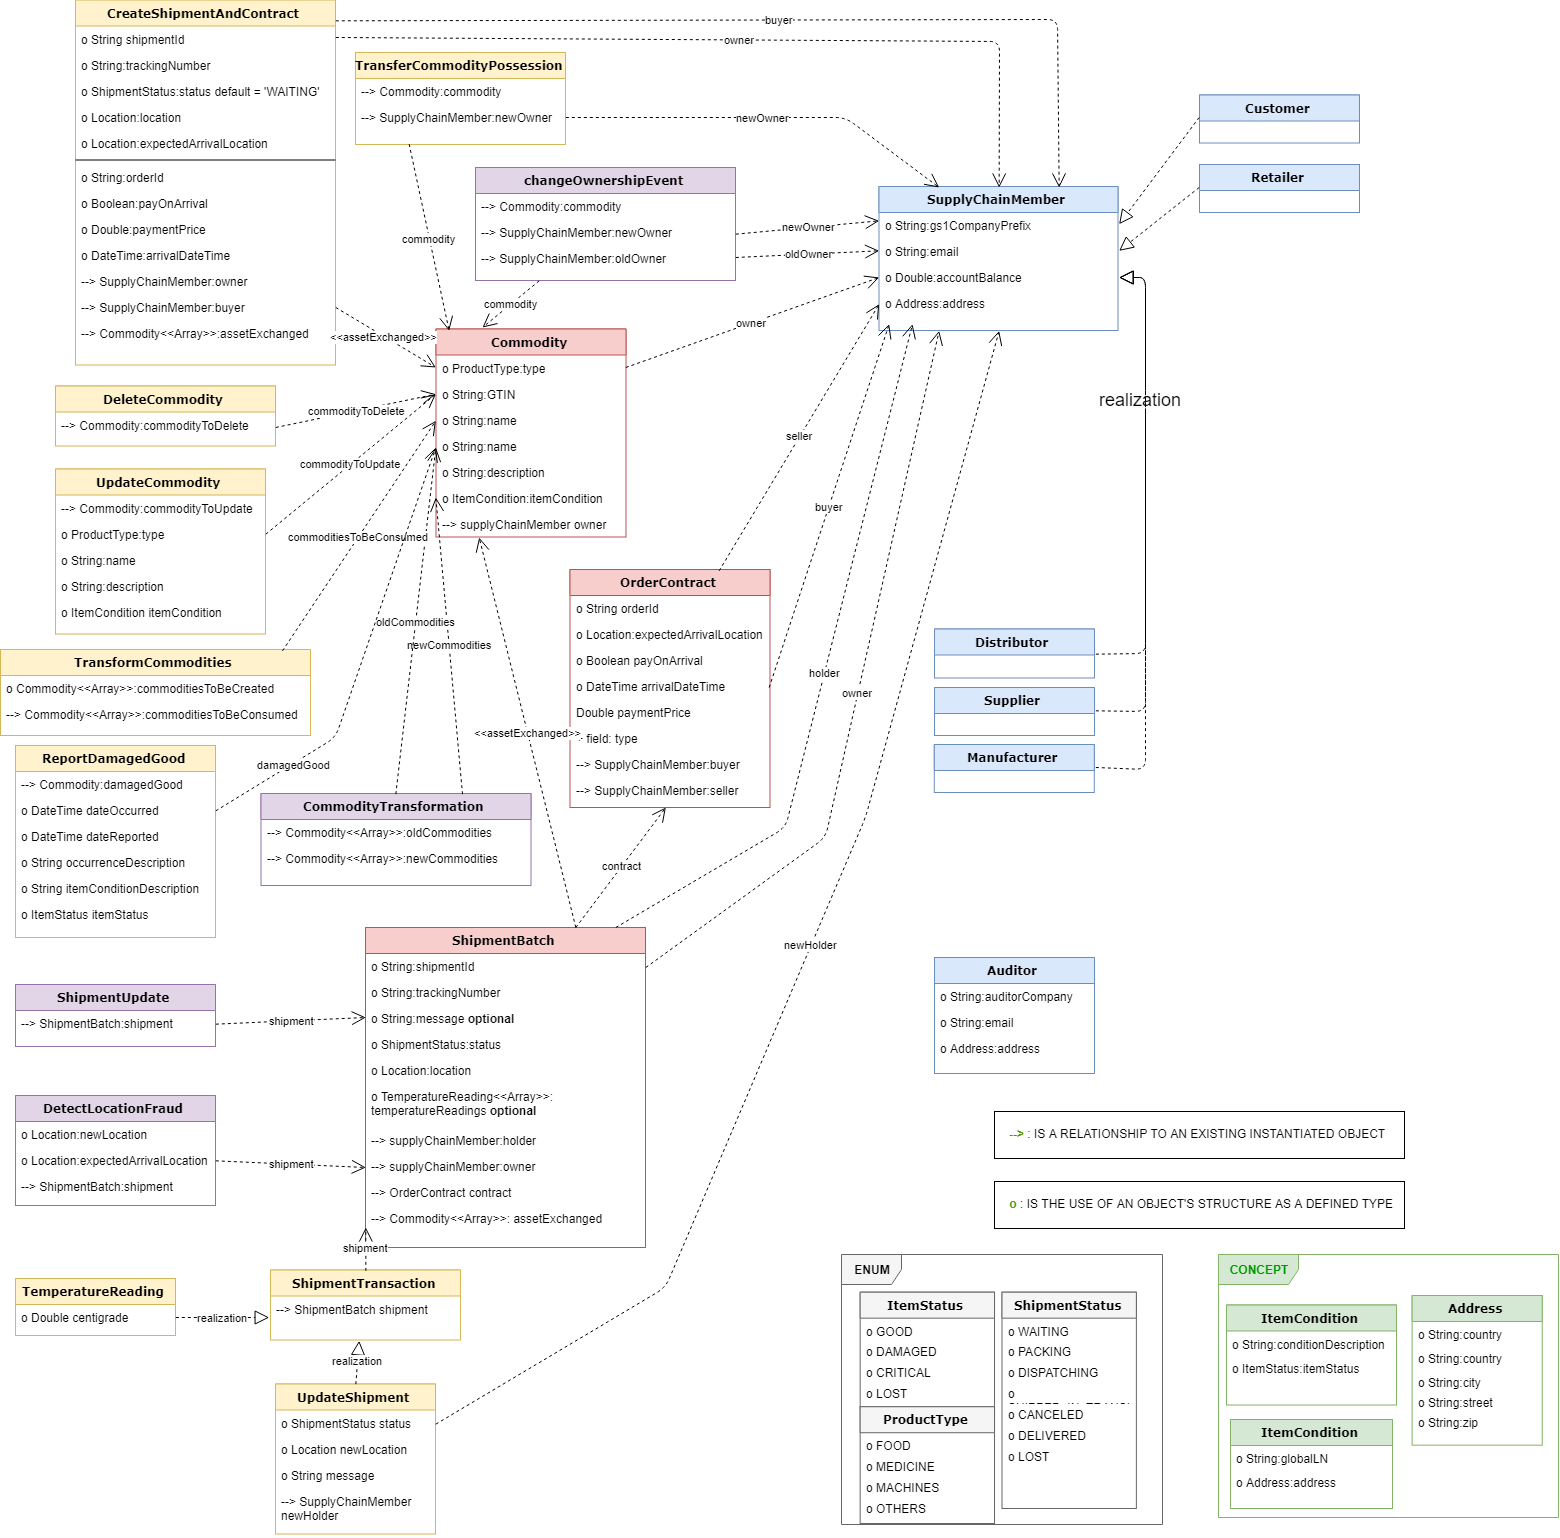
\includegraphics[scale=0.32]{media/full_class_diagram.png}
    \caption[Full class diagram for the designed Hyperledger Composer model]{Full class diagram for the designed Hyperledger Composer model}
    \label{fig:full_class_diagram}
\end{figure}



	% seealso index entries (must come after all other \index calls, so that they appear as the last subitems on index entries)
	%\index{knowledge!capture|seealso{expressiveness}}
	%\index{information|seealso{knowledge, capture}}

	
	\bookmarksetup{startatroot}
	\backmatter
		\cleardoublepage
		\chapter{Publications}
\label{chap:publications}

Many of the materials in this thesis have appeared in the following publications.

\section*{Peer-reviewed Conference Papers}

Lorem ipsum.

\section*{Peer-reviewed Journal Papers}

Lorem ipsum.

\section*{Peer-reviewed Workshop Papers}

Lorem ipsum.

\section*{Peer-reviewed Posters}

Lorem ipsum.

\section*{Doctoral Symposiums}

Lorem ipsum.



		% Glossary
		%\cleardoublepage
		%\phantomsection
		%\begin{singlespace}
		%\begin{footnotesize}
		%\addcontentsline{toc}{chapter}{Nomenclature}
		%\markboth{Nomenclature}{Nomenclature}
		%\makenomenclature
		%% !TEX root = ../thesis.tex

\chapter*{Nomenclature}
\chaptermark{NOMENCLATURE}


\begin{flushleft}
\begin{tabular}{l p{0.8\linewidth}}
	ABB  & Abbreviation
\end{tabular}
\end{flushleft}

		%\printnomenclature[4.5cm]
		%\end{footnotesize}
		%\end{singlespace}

		% Bibliography / References
		\cleardoublepage
		\phantomsection
		\begin{singlespace}
		\begin{footnotesize}
		\addcontentsline{toc}{chapter}{References}
		\bibliographystyle{amsalpha}
		\renewcommand{\bibname}{References}
		\bibliography{references}
		\end{footnotesize}
		\end{singlespace}
		\cleardoublepage
		\phantomsection
		\addcontentsline{toc}{chapter}{Index}
		\printindex
\end{document}
